\section{The Class Buffer Model}

As a result of the challenges in the perception of classes and the separation of clusters the designers of maps face various tasks to convey the correct idea to support their data. A cluster has to be well fitted into the graph to show the information in a comprehensible way. These problems can be considered each on their own but also intertwined as a whole. This is where the class buffer model comes to action.

In many approaches the designers have to think of different data aggregation, dimension reduction, visual encoding or rendering methods and know the advantages of many. The challenge of visualizing different approaches beforehand to have a mental image when creating density maps lead to the implementation of the Class Buffer model. This model takes the designer through a interactive approach to visualize data in multiclass density maps.

\begin{figure}
  \centering
	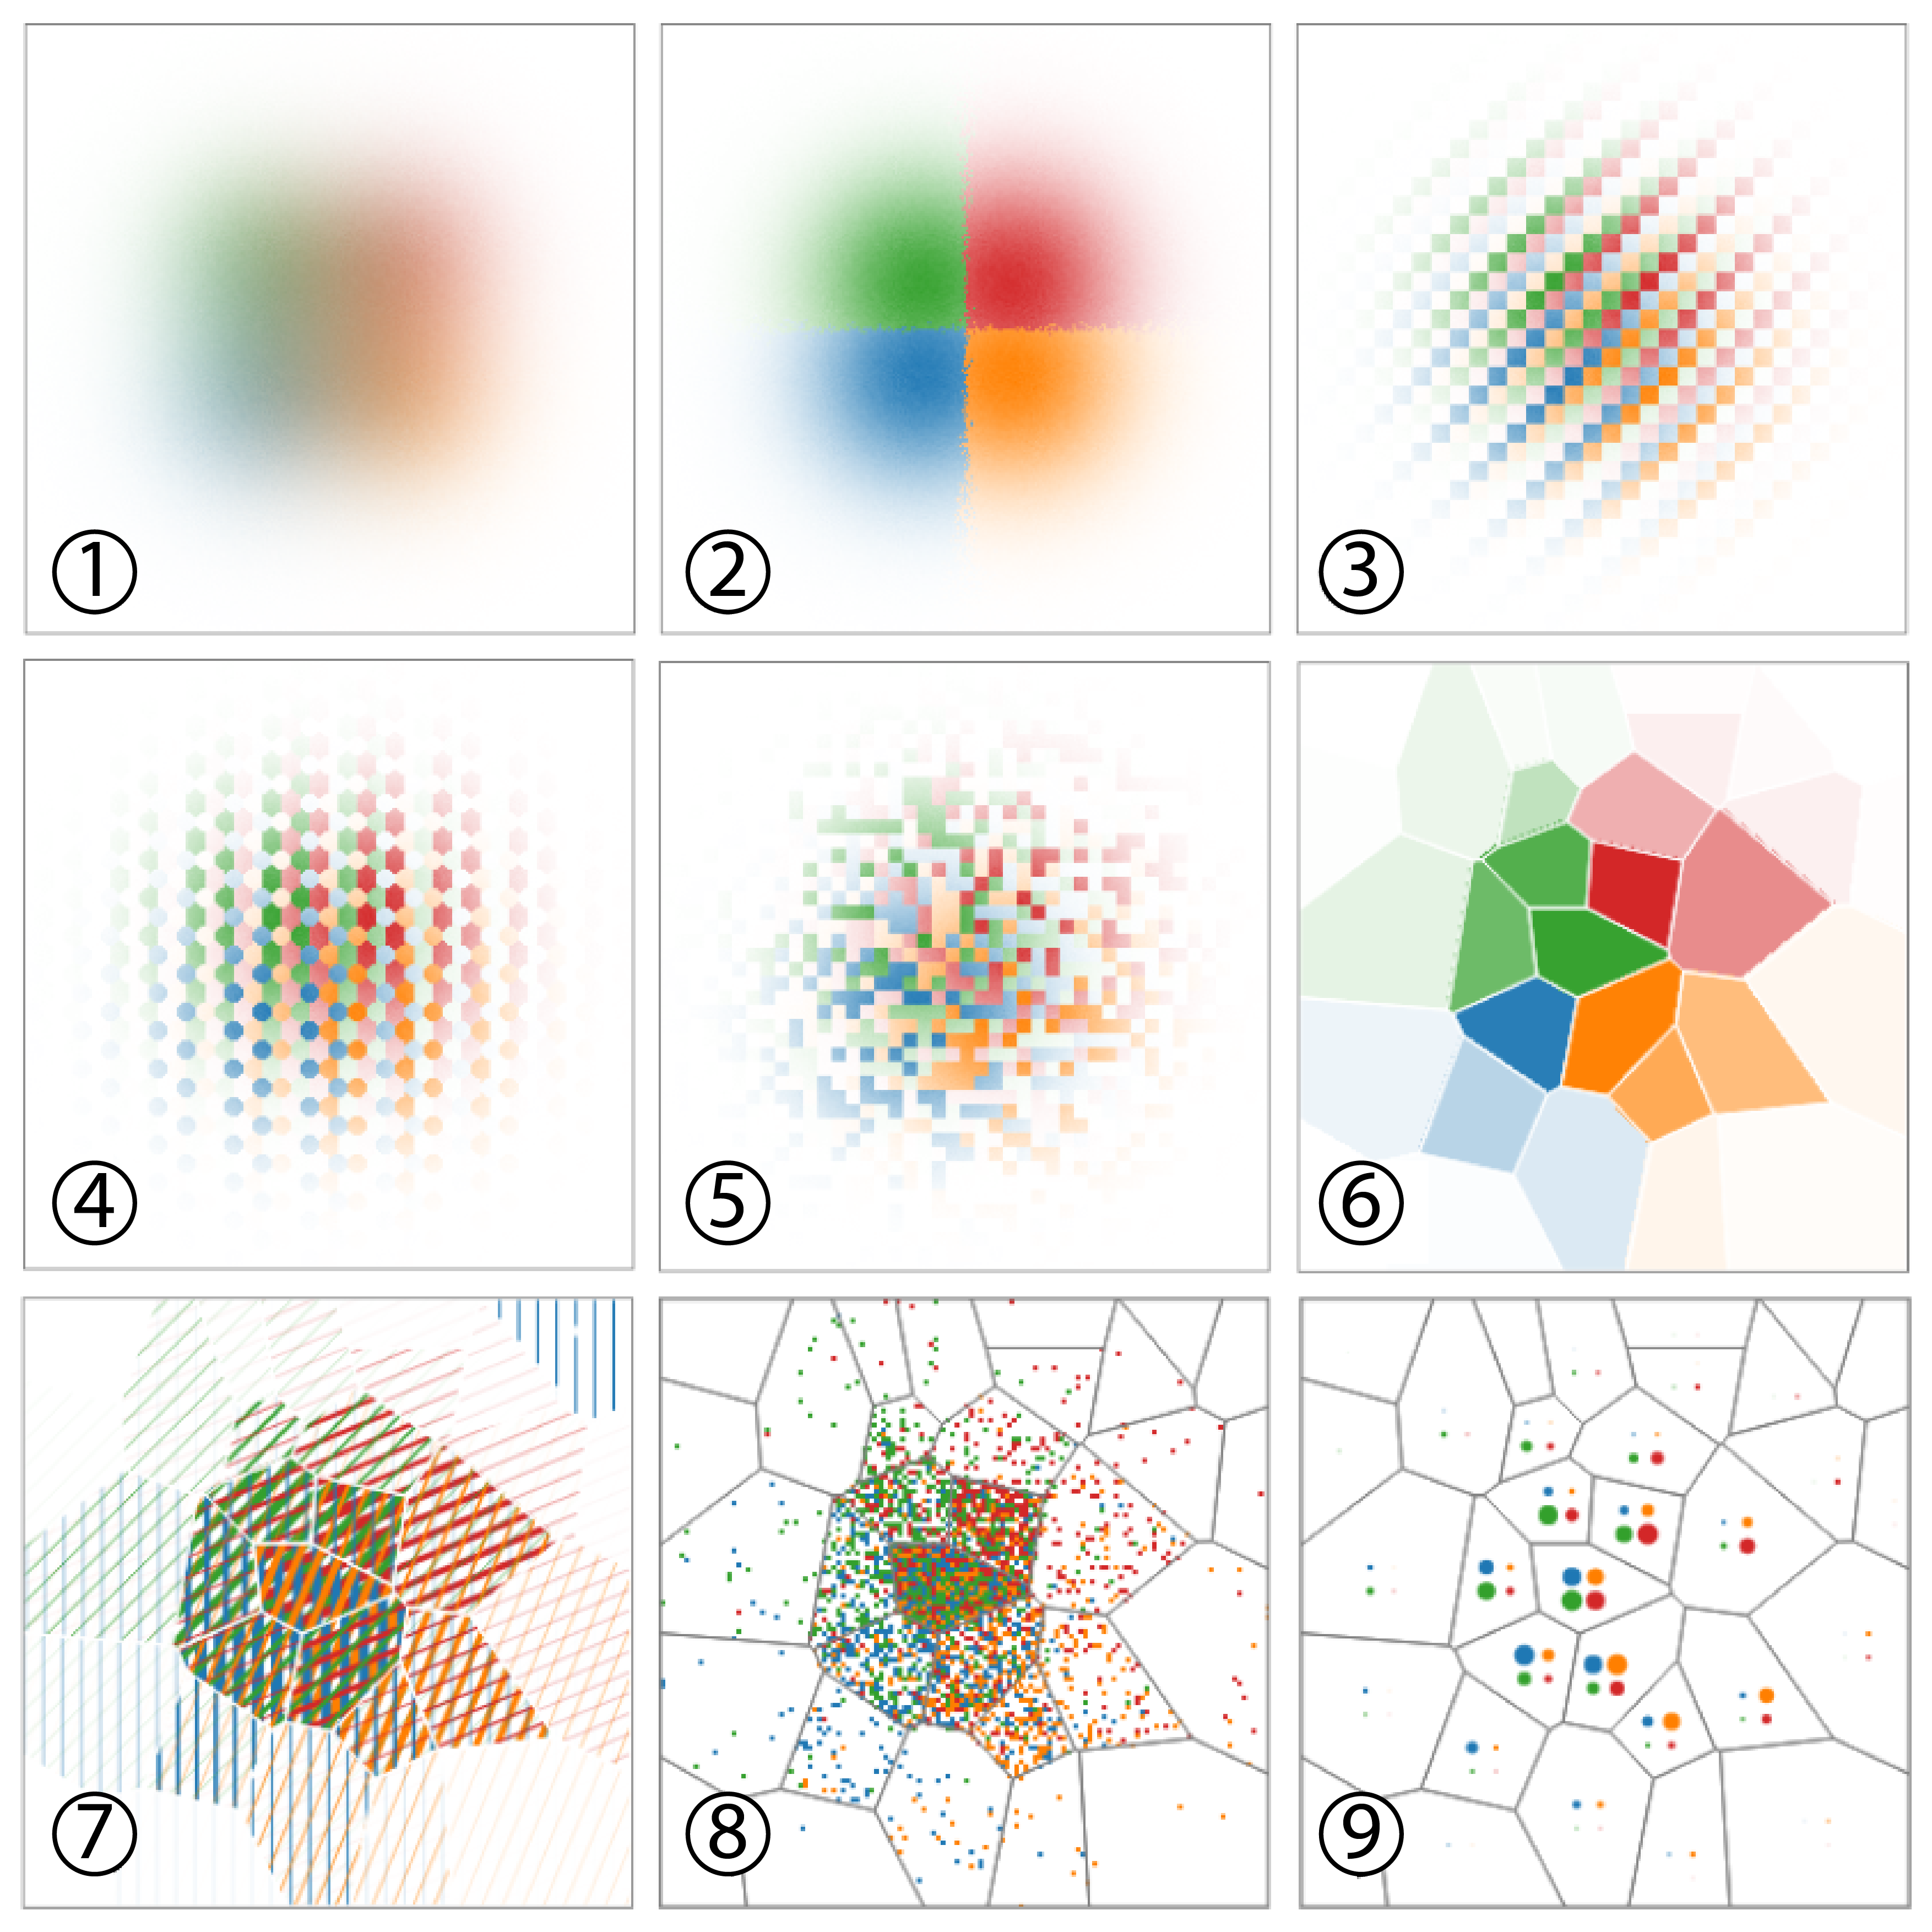
\includegraphics[width=\columnwidth]{./figures/results}
	\caption{A few results generated from the Class Buffer model. 1. Blending of the density maps. 2. winner-takes-all approach. The class with the highest count is chosen. 3. - 5. Three different weaving patterns. 3. and 4. are regular patterns, 5. is an irregular weaving pattern. 6. - 9. Uses rebinning (binning and aggregation over the density maps) with tiles produced by a random Voronoi pattern. 6. Shows the highest count in the tile, 7. Shows hatching, 8. shows a dot density plot, 9. Shows a punch card.\\\textcopyright~Extracted from \textit{A Declarative Rendering Model for Multiclass Density Maps} and digitally edited, Jo et al.,~\cite{jo2019declarative}}\label{fig:mdm-results}
\end{figure}

\begin{figure*}
	\centering
	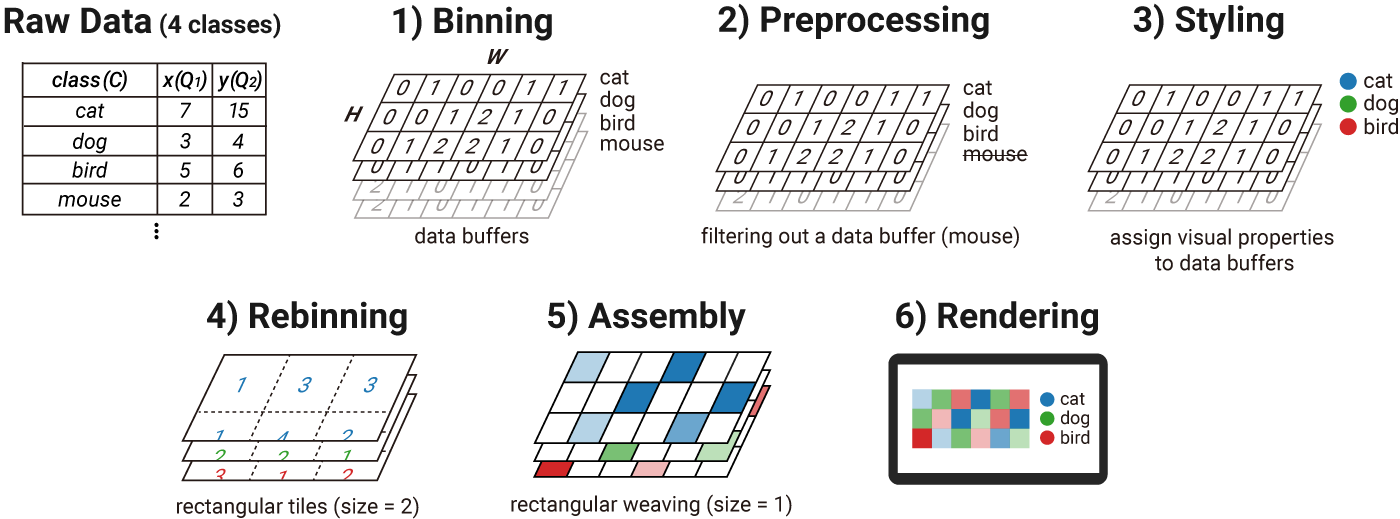
\includegraphics[width=0.85\textwidth]{./figures/Multiclass_Density_Maps-10}
	\caption{The six stages of the Class Buffer model. First binning, the data is split into as many data buffers as tables.$\star$ Second the preprocessing, like gaussian smoothing.$\bullet$ Third styling where the data buffers are assigned i.e. colors.$\bullet$ Fourth rebinning where the classes get partitioned into tiles, aggregated and normalized.$\bullet$ Fifth the assembly where tiles and normalized counts are turned into a single density map.$\bullet$ Sixth the rendering of the data, here legends axis and landmarks etc. are added for better understanding of the visualization.$\bullet$\\$\star$: Done in the back-end.$\bullet$: Done in the front-end. \textcopyright~Extracted from \textit{A Declarative Rendering Model for Multiclass Density Maps}, Jo et al.,~\cite{jo2019declarative}}\label{fig:mdm-stages}
\end{figure*}

The Class Buffer model is implemented to use the JSON data-interchange format. It defines an expressive visualization grammar for multiclass density maps, the specification of this grammar can be seen in Listing~\ref{lis:specs}. The Class Buffer model is based on the Class Buffer idiom~\cite{chen2018using} as the primary building block.
The implementation of the Class Buffer model from Jo et al. consists of six stages, that are apportioned to either the back-end that is processing much of the data or the front-end of the system displaying the data. This approach comes from the advantages of the specification, where tasks can easily be implemented on both sides of modern web applications. The back-end is responsible and capable of doing larger calculations and the front-end is dedicated to filtering, styling and displaying the data. The six stages used in the model can be seen in Figure~\ref{fig:mdm-stages} and are described as follows:

\begin{enumerate}[leftmargin=*]
	\setlength\itemsep{0.1em}
	\item \textbf{Binning.} Data that is given into the system is divided into data buffers where the number of data buffers corresponds to the number of classes in the data. A data buffer can be understood as a 2D histogram that counts the occurrence of a data case and groups those belonging together. This binning is implemented in the backend of the system because it consists of only semantic calculations and no styling. The backend will transfer the data buffers to the front-end where the second and following steps will take place.\\The main goal of doing this step on the back-end side is to enable the rendering to happen in interactive time~\cite{jo2019declarative} and because this step has to be done generally only once for the lifecycle of a map. By doing so the model supports stationary as well as handheld devices and their respective computational power.
	\item \textbf{Preprocessing.} When the data buffers get passed to the front-end of the application a preprocessing operation is realized. This preprocessing is most often a gaussian smoothing over each buffer individually. Smoothing allows the elimination of problems with excessive variability in the summaries~\cite{wickham2013bin}.\\Data can likewise be filtered by different properties and criteria that should be left out of the rendering process. Combinations of different data buffers can moreover be created. Because of this filtering and combining data into mixed data buffers the preprocessing step is done in the front-end to eliminate expensive round trips when filters change.
	\item \textbf{Styling.} The first styling step performed is a transformation from data buffers to class buffers. Class buffers represent the same separated data as data buffers but with additional information such as class specific color, hatching angle or scale.\\These visual properties are specified on the front-end using the grammar of the Class Buffer model, as described by Jo et al.~\cite{jo2019declarative} can be seen in Listing~\ref{lis:specs}.
	\item \textbf{Rebinning.} The front-end then partitions the class buffers, that is divided into grids, into tiles. These can be equidistant partitions of the two dimensional domain that the data resides in, but also a more irregular divided separation of space like a Voronoy separation. An important property is that the tiling is defined so that there is no overlapping within them. Additionally an aggregated count is computed for each class and stored in a data vector. This aggregation is all pixels from class \textit{i} that belong to the tile \textit{t}. It is afterwards normalized to a value between 0 and 1 using a linear, log, square root or equi-depth histogram scale to be used in the legend.
	\item \textbf{Assembly.} Tiles and normalized data vectors are turned into a single density map image. This step adds more styling to the process, like an alpha channel, and different approaches to unify the maps are possible, namely, masking, mixing, hatching, and generating glyphs based on the aggregated count described below.\\\textbf{Masking} is the process where a mask is assigned to each class buffer. This mask is a grid of the same size as the original grid and is defined such that the sum of every mask grid equals 1 for each pixel. Then each tile is rendered for each class buffer with a uniform color previously assigned in the styling stage and the corresponding opacity value of the normalized count stored in the data vector. The resulting image is then alpha-blended using the opacity values stored in the mask. This approach is used for the weaving pattern that can be seen in Figure~\ref{fig:mdm-results} in example 3 and 4.\\The \textbf{Mixing} operation on the other hand combine tiles by blending them. The main goal is to receive a resulting image that is similar to the one generated by masking but with colors that are blended across the entire tile instead of being masked. Different mixing methods can be used, in example \textit{additive mixing} sums each RGB channel of the colors, thus generating brighter colors as \textit{multiplicative mixing}, which generates darker colors for high density regions. Additionally, it is possible to take an \textit{winner-takes-all} or \textit{loser-takes-all} approach where either the class with the highest or lowest count is chosen.\\Tiles can furthermore be rendered by using the \textbf{hatching} operation, which fills each tile with evenly spaced lines. Typically the line thickness encodes the normalized count, while the line orientation encodes the class. The hatches can be combined by stacking them side by side within each or by superimposing them, like in Figure~\ref{fig:mdm-results}, example 7.\\A more conventional pipeline is \textbf{glyph generation} to visualize the previously processed data. Glyphs are miniature visualizations that are used to encode the normalized counts of the data and are typically rendered in the center of the tile, like in Figure~\ref{fig:mdm-results}, in example 8 and 9. The position can be slightly moved to make space for glyphs from other classes. This can result in visualizations like a punch card or the mixture of bar chart and density map where each tile in the visualization holds a bar chart indicating the normalized value of the data.\\Jo et al.~\cite{jo2019declarative} compute the position of the glyph as the largest rectangle in polygon for each tile and place the glyph in the middle of this rectangle. This assembly step might be the most comprehensive step of the Class Buffer model but it is optional as well. When no assembly operation is specified, each tile is rendered using a uniform translucent color, and the process outputs multiple density map images instead of a single one, leaving the conflict resolution to the final rendering stage.
	\item \textbf{Rendering.} The final step shows the single density map on the medium the user desires, either stationary or handheld devices, such as mobile phones. The background color of the plot defines the lower end of the color scale used in the visualization. For example, a white background will result in a color scale where white is indicating the lowest, or zero density. Black backgrounds will produce the same effect but might have other (dis-)advantages. The background does not have to be of uniform color but can also show cartographic or other information.\\In this stage a variety of helping decorations and annotations can be added, i.e. landmarks and axes, to make the visualization easier to understand by the viewer and a legend can be added to complete the visualization process.
\end{enumerate}

\blfootnote{The implementation form Jo et al. is available, with example datasets, at \url{https://github.com/e-/Multiclass-Density-Maps} and examples can additionally be explored at \url{https://jaeminjo.github.io/Multiclass-Density-Maps/}.}

The Class Buffer model is implemented in TypeScript, a strongly typed language that can be transpiled into JavaScript, which runs in every modern browser as basis of the dynamic web.
Additionally, the implementation relies on the D3 library for contours and cartographic projections.
Interpreting a specification takes between a few hundred milliseconds to one second depending on the complexity of the operations to perform~\cite{jo2019declarative}, not counting the time to transfer the data, including data buffers. 

In the implementation of the class buffer model, glyphs can be specified in Vega-Lite~\cite{satyanarayan2016vega}, a high-level JSON grammar for interactive graphics. It provides a concise JSON syntax for rapidly generating visualizations to support analysis.

Tiles can be defined based on geometrical primitives or using the URI of a TopoJSON~\cite{online:topojson} specification to define geographic administrative boundaries. TopoJSON is an extension of GeoJSON that encodes topology. Rather than representing geometries discretely, geometries in TopoJSON files are stitched together from shared line segments. TopoJSON eliminates redundancy, allowing related geometries to be stored efficiently in the same file.

Changing a specification and reinterpreting data is generally a lot quicker as information isn't changed. Intermediate operations, such as rebinning, can be cached if the tiling is not changed, which is common for geographical maps~\cite{jo2019declarative}.
Tile glyphs are rendered using Vega-Lite~\cite{satyanarayan2016vega}.

% \begin{minipage}[0mm]{\columnwidth}
\begin{lstfloat}
	\small{
		\begin{lstlisting}[caption={Syntax of Class Buffer specifications. Different TypeScript notations show the required JSON fields for the model to interpret the data in the minimal way~\cite{jo2019declarative}. Fields denoted by questionmarks can be omitted.},captionpos=b,label=lis:specs]
{"description"?: <string>,
"background"?: <Color>,
"data": {"url": <url> | "dataSpec": <DataSpec>},
"smooth"?: {"radius": <number>},
"reencoding"?: {
  "label"?: <LabelSpec>, "color"?: <ColorSpec>,
  "hatching"?: <HatchingSpec>
},
"rescale"?: {
  "type": "linear" | "log" | "pow" | 
          "sqrt" | "cbrt" | "equidepth",
  "rebin"?: {
      "type": "none" | "square" | "rect" | "topojson" | 
              "voronoi",
      "aggregation": "mean" | "max" | "sum" | "min" | 
              "density",
      "width"?: <number>, "height"?: <number>,
      "size"?: <number>, "topojson"?: <TopoJSONSpec>,
      "url"?: <string>, "feature"?: <string>,
      "points"?: <Point[]>, "stroke"?: <Color>
  },
  "compose"?: {
    "mix": "none" | "invmin" | "mean" | "max" | "blend" | 
           "weavingrandom" | "weavingsquare" | 
           "weavinghex" | "weavingtri" | "propline" | 
           "hatching" | "separate" | "glyph" | 
           "dotdensity" | "time",
    "mixing"?: "additive" | "subtractive" | 
               "multiplicative",
    "size"?: <number>, "widthprop"?: <string|number>,
    "colprop"?:<boolean>, "order"?: <number[]>,
    "glyphSpec"?: <GlyphSpec>, "interval"?: <number>
  },
  "levels"?: <number>
},
"contour"?: {
  "stroke": <number>, "lineWidth"?: <number>,
  "values"?: <number[]>, "blur"?: <number>
},
"legend"?: <LegendSpec>, "stroke"?: <StrokeSpec>,
"axis"?: <AxisSpec>}
\end{lstlisting}
	}
\end{lstfloat}

\subsection{Benefits of the Class Buffer model}
The Class Buffer model is more scalable over the three facets, data size, perceptual processing, and computation speed when compared with other frameworks for visualizing large maps~\cite{jo2019declarative}. This is largely due to the separation of computational tasks between the back-end and the front-end in the implementation.
The back-end side computes density maps, which will result in proportional computation time in relation to the number of points.
Once this expensive computation is done, the visualizations offered by the model can be used to explore the data at 'interactive' speed, regardless of the size of the original data.
Jo et al.~\cite{jo2019declarative} argue that it can be about millions, billions, or any higher scale of data points.

Other visualization libraries compute the aggregation and the visualization together, needing a time proportional to the number of points to generate a new visualization and require expensive round-trips from the back-end to the browser. Abstract Rendering~\cite{cottam2013overplotting, cottam2014abstract} performs the binning operations in complex buffers that are configured early before their contents are computed.
Once computed, most of the rendering has to be performed in the back-end as well because the composite structure at each bin is structured in a way that a transparent transmission to a front-end for easy visualization becomes impractical. Each modification of the pipeline requires an expensive recomputation starting at the binning stage, requiring the handling of the whole dataset.

By contrast, the Class Buffer model receives the raw unsmoothed density map and can apply a smoothing kernel to it at its first stage. According to Wickham~\cite{wickham2013bin}, applying the smoothing to the binned data produces very similar results than applying it before binning, with a substantial performance improvement~\cite{wand1994fast}. Compared with Wickham’s BSS model~\cite{wickham2013bin}, the Class Buffer model provides a richer set of visualization options, but less statistical operations at the prebinning stage. This is because the BSS model does not manage multiclass data.

% Copmposing multiple classes from density maps is understandable since densities are directly comparable, but with more complex statistics such as average, variance, or higher-order moments, the interpretations of the class combinations are challenging.

\subsection{Interactive Data Exploration}

The Class Buffer model uses 2D histograms, calculated from data buffers, as data sources. This provides the model with the ability to abstract the underlying computation of large-scale data~\cite{jo2019declarative}.
When the dataset is filtered by a new dimension, the data buffers should be invalidated and recomputed. Because of the changes in the filtering all binning could be changed, which results in the need for completely new data aggregated by different properties. 
In interactive exploration with multidimensional data, this would be a frequent case, and modern data structures~\cite{lins2013nanocubes, liu2013immens} have been proposed to speed up the recomputation. The Class Buffer model naturally lends itself to working with those optimized data structures through the transfer of \textit{abstract} data buffers between the front- and back-end of the system. The model uses this method in order to facilitate a dynamic change of visualization types in real time on all devices. The user can, by using this system, view multiple variants of visualizations for the same group of data bins.\\ 
In addition, the ProgressiVis toolkit~\cite{fekete2016progressive} already transfers data buffers of progressively aggregated data to its front-end, which can be used with the Class Buffer model.

% \textcolor{red}{\lipsum[2]}

\subsection{Limitations}

A wide variety of visualizations, suited to complex tasks, can be created using the Class Buffer model. These visualizations show the complex data in a way that the viewer might comprehend coherences more easily and with less cognitive effort than visualizations created by hand. They almost always need additional information to be fully comprehensible, such as landmarks, points of interest, and marks of outliers. The depiction, because of the binning, masking and mixing, additionally needs a legend.
Landmarks for maps include important locations and names, sometimes additional shapes to add context, such as rivers or points of interest. Landmarks for scatterplots and multidimensional projections include location of interesting points.
For example, in publication data, highly cited publications or authors can be used as landmarks.
All these additional guides should be combined and added to the image at the rendering stage.

The Class Buffer model can replicate several techniques used to visualize multiclass density maps, but it does not offer guidance on their best use. 
By providing this implementation Jo et al.~\cite{jo2019declarative} enable the visualization community to continue researching multiclass density maps, opening up a new area of scalable visualization. 
